\setmodule{9}

%BEGIN_FOLD % ====>>_____ Занятие 1 _____<<====
\begin{class}[number=1]
	\begin{listofex}
		%11.2,3,4 по 3 первых
		\item Найдите точку максимума функции \(y=x^3-48x+17\).
		\item Найдите наименьшее значение функции \(y=x^3-27x\) на отрезке \([0;4]\).
		\item Найдите наибольшее значение функции \(y=x^3-3x+4\) на отрезке \([-2;0]\).
		\item Найдите точку максимума функции \(y=-\dfrac{ x^2+289 }{ x }\).
		\item Найдите точку минимума функции \(y=-\dfrac{ x^2+1 }{ x }\).
		\item Найдите наименьшее значение функции \(y=\dfrac{ x^2+25 }{ x }\) на отрезке \([1;10]\).
		\item Найдите наименьшее значение функции \(y=(x-8)e^{x-7}\) на отрезке \([6;8]\).
		\item Найдите точку минимума функции \(y=(x+16)e^{x-16}\).
		\item Найдите точку максимума функции \(y=(9-x)e^{x+9}\).
		\item Изюм получается в процессе сушки винограда. Сколько килограммов винограда потребуется для получения \(20\) килограммов изюма, если виноград содержит \(90\%\) воды, а изюм содержит \(5\%\) воды?
		%\item Изюм получается в процессе сушки винограда. Сколько килограммов винограда потребуется для получения \(16\) килограммов изюма, если виноград содержит \(90\%\) воды, а изюм содержит \(5\%\) воды?
		%BANK https://math-ege.sdamgia.ru/test?likes=99575 // https://math-ege.sdamgia.ru/test?likes=99576 // https://math-ege.sdamgia.ru/test?likes=99576 // https://math-ege.sdamgia.ru/test?likes=99578
		%по 2
		\item Имеется два сплава. Первый сплав содержит \(5\%\) меди, второй --- \(12\%\) меди. Масса второго сплава больше массы первого на \(9\) кг. Из этих двух сплавов получили третий сплав, содержащий \(10\%\) меди. Найдите массу третьего сплава. Ответ дайте в килограммах.
		%\item Имеется два сплава. Первый сплав содержит \(5\%\) меди, второй --- \(13\%\) меди. Масса второго сплава больше массы первого на \(9\) кг. Из этих двух сплавов получили третий сплав, содержащий \(10\%\) меди. Найдите массу третьего сплава. Ответ дайте в килограммах.
		
		\item Смешав \(11\)-процентный и \(72\)-процентный растворы кислоты и добавив \(10\) кг чистой воды, получили \(31\)-процентный раствор кислоты. Если бы вместо \(10\) кг воды добавили \(10\) кг \(50\)-процентного раствора той же кислоты, то получили бы \(51\)-процентный раствор кислоты. Сколько килограммов \(11\)-процентного раствора использовали для получения смеси?
		%\item Смешав \(55\)-процентный и \(97\)-процентный растворы кислоты и добавив \(10\) кг чистой воды, получили \(65\)-процентный раствор кислоты. Если бы вместо \(10\) кг воды добавили \(10\) кг \(50\)-процентного раствора той же кислоты, то получили бы \(75\)-процентный раствор кислоты. Сколько килограммов \(55\)-процентного раствора использовали для получения смеси?
		
		%\item Имеется два сплава. Первый содержит \(10\%\) никеля, второй --- \(35\%\) никеля. Из этих двух сплавов получили третий сплав массой \(150\) кг, содержащий \(30\%\) никеля. На сколько килограммов масса первого сплава была меньше массы второго?
		\item Имеется два сплава. Первый содержит \(15\%\) никеля, второй --- \(35\%\) никеля. Из этих двух сплавов получили третий сплав массой \(140\) кг, содержащий \(30\%\) никеля. На сколько килограммов масса первого сплава была меньше массы второго?
		
		
		\item Имеются два сосуда. Первый содержит \(30\) кг, а второй --- \(15\) кг раствора кислоты различной концентрации. Если эти растворы смешать, то получится раствор, содержащий \(34\%\) кислоты. Если же смешать равные массы этих растворов, то получится раствор, содержащий \(46\%\) кислоты. Сколько килограммов кислоты содержится в первом сосуде?
		%\item Имеются два сосуда. Первый содержит \(100\) кг, а второй --- \(20\) кг раствора кислоты различной концентрации. Если эти растворы смешать, то получится раствор, содержащий \(67\%\) кислоты. Если же смешать равные массы этих растворов, то получится раствор, содержащий \(77\%\) кислоты. Сколько килограммов кислоты содержится в первом сосуде?
	\end{listofex}
\end{class}
%END_FOLD

%BEGIN_FOLD % ====>>_____ Занятие 2 _____<<====
\begin{class}[number=2]
	\begin{listofex}
		%11.2,3 по 4-5 И 11.4 3 первых
		\item Найдите точку максимума функции \(y=x^3-3x^2+2\).
		\item Найдите точку минимума функции \(y=2x^3-5x^2+1\).
		\item Найдите наибольшее значение функции \(y=\dfrac{ x^2+25 }{ x }\) на отрезке \([-10;-1]\).
		\item Найдите точку максимума функции \(y=\dfrac{ 16 }{x  }+x+3\).
		\item Найдите наименьшее значение функции \(y=(x-8)e^{x-7}\) на отрезке \([6;8]\).
		\item Найдите точку минимума функции \(y=(x+16)e^{x-16}\).
		\item Найдите точку максимума функции \(y=(9-x)e^{x+9}\).
		%по 2
		\item Имеется два сплава. Первый сплав содержит \(5\%\) меди, второй --- \(12\%\) меди. Масса второго сплава больше массы первого на \(9\) кг. Из этих двух сплавов получили третий сплав, содержащий \(10\%\) меди. Найдите массу третьего сплава. Ответ дайте в килограммах.
		%\item Имеется два сплава. Первый сплав содержит \(5\%\) меди, второй --- \(13\%\) меди. Масса второго сплава больше массы первого на \(9\) кг. Из этих двух сплавов получили третий сплав, содержащий \(10\%\) меди. Найдите массу третьего сплава. Ответ дайте в килограммах.
		
		\item Смешав \(11\)-процентный и \(72\)-процентный растворы кислоты и добавив \(10\) кг чистой воды, получили \(31\)-процентный раствор кислоты. Если бы вместо \(10\) кг воды добавили \(10\) кг \(50\)-процентного раствора той же кислоты, то получили бы \(51\)-процентный раствор кислоты. Сколько килограммов \(11\)-процентного раствора использовали для получения смеси?
		%\item Смешав \(55\)-процентный и \(97\)-процентный растворы кислоты и добавив \(10\) кг чистой воды, получили \(65\)-процентный раствор кислоты. Если бы вместо \(10\) кг воды добавили \(10\) кг \(50\)-процентного раствора той же кислоты, то получили бы \(75\)-процентный раствор кислоты. Сколько килограммов \(55\)-процентного раствора использовали для получения смеси?
		
		%\item Имеется два сплава. Первый содержит \(10\%\) никеля, второй --- \(35\%\) никеля. Из этих двух сплавов получили третий сплав массой \(150\) кг, содержащий \(30\%\) никеля. На сколько килограммов масса первого сплава была меньше массы второго?
		\item Имеется два сплава. Первый содержит \(15\%\) никеля, второй --- \(35\%\) никеля. Из этих двух сплавов получили третий сплав массой \(140\) кг, содержащий \(30\%\) никеля. На сколько килограммов масса первого сплава была меньше массы второго?
		
		
		\item Имеются два сосуда. Первый содержит \(30\) кг, а второй --- \(15\) кг раствора кислоты различной концентрации. Если эти растворы смешать, то получится раствор, содержащий \(34\%\) кислоты. Если же смешать равные массы этих растворов, то получится раствор, содержащий \(46\%\) кислоты. Сколько килограммов кислоты содержится в первом сосуде?
		%\item Имеются два сосуда. Первый содержит \(100\) кг, а второй --- \(20\) кг раствора кислоты различной концентрации. Если эти растворы смешать, то получится раствор, содержащий \(67\%\) кислоты. Если же смешать равные массы этих растворов, то получится раствор, содержащий \(77\%\) кислоты. Сколько килограммов кислоты содержится в первом сосуде?
	\end{listofex}
\end{class}
%END_FOLD

%BEGIN_FOLD % ====>>_ Домашняя работа 1 _<<====
\begin{homework}[number=1]
	\begin{listofex}
		%11.2,3 по 6-7 И 11.4 4-5
		\item Найдите наименьшее значение функции \(y=x^3-3x^2+2\) на отрезке \([1;4]\).
		\item Найдите наибольшее значение функции \(y=x^3-6x^2\) на отрезке \([-3;3]\).
		\item Найдите точку минимума функции \(y=\dfrac{ 25 }{ x }+x+25\).
		\item Найдите точку максимума функции \(y=-\dfrac{ x }{ x^2+9 }\).
		\item Найдите точку минимума функции \(y=(3-x)e^{3-x}\).
		\item Найдите наибольшее значение функции \(y=(x+16)e^{16-x}\) на отрезке \([15;17]\).
		\item Изюм получается в процессе сушки винограда. Сколько килограммов винограда потребуется для получения \(82\) килограммов изюма, если виноград содержит \(90\%\) воды, а изюм содержит \(5\%\) воды?
		\item Два промышленных фильтра, работая одновременно, очищают цистерну воды за \(30\) минут. Определите, за сколько минут второй фильтр очистит цистерну воды, работая отдельно, если известно, что он сделает это на \(25\) минут быстрее, чем первый.
	\end{listofex}
\end{homework}
%END_FOLD

%BEGIN_FOLD % ====>>_____ Занятие 3 _____<<====
\begin{class}[number=3]
	\begin{listofex}
		%11.4 7-9 И 11.5 1-4
		\item Найдите точку максимума функции \( y=(3x^2-36x+36)e^{x+36}. \)
		\item Найдите точку максимума функции \(y=(x^2-10x+10)e^{5-x}\).
		\item Найдите точку максимума функции \(y=(x-2)^2e^{x-6}\).
		\item Найдите наибольшее значение функции \(y=8\ln(x+7)-8x+3\) на отрезке \([-6,5; 0]\).
		\item Найдите наименьшее значение функции \(y=4x-4\ln(x+7)+6\) на отрезке \([-6,5; 0]\).
		\item Найдите наибольшее значение функции \(y=\ln(x+5)^5-5x\) на отрезке \([-4,5; 0]\).
		\item Найдите наименьшее значение функции \(y=3x-\ln(x+3)^3\) на отрезке \([-2,5; 0]\).
		
		
		
		%BANK https://math-ege.sdamgia.ru/test?likes=99575 // https://math-ege.sdamgia.ru/test?likes=99576 // https://math-ege.sdamgia.ru/test?likes=99576 // https://math-ege.sdamgia.ru/test?likes=99578
		%по 2
		\item Имеется два сплава. Первый сплав содержит \(5\%\) меди, второй --- \(12\%\) меди. Масса второго сплава больше массы первого на \(9\) кг. Из этих двух сплавов получили третий сплав, содержащий \(10\%\) меди. Найдите массу третьего сплава. Ответ дайте в килограммах.
		%\item Имеется два сплава. Первый сплав содержит \(5\%\) меди, второй --- \(13\%\) меди. Масса второго сплава больше массы первого на \(9\) кг. Из этих двух сплавов получили третий сплав, содержащий \(10\%\) меди. Найдите массу третьего сплава. Ответ дайте в килограммах.
		
		\item Смешав \(11\)-процентный и \(72\)-процентный растворы кислоты и добавив \(10\) кг чистой воды, получили \(31\)-процентный раствор кислоты. Если бы вместо \(10\) кг воды добавили \(10\) кг \(50\)-процентного раствора той же кислоты, то получили бы \(51\)-процентный раствор кислоты. Сколько килограммов \(11\)-процентного раствора использовали для получения смеси?
		
		
		%\item Имеется два сплава. Первый содержит \(10\%\) никеля, второй --- \(35\%\) никеля. Из этих двух сплавов получили третий сплав массой \(150\) кг, содержащий \(30\%\) никеля. На сколько килограммов масса первого сплава была меньше массы второго?
		
		%\item Имеются два сосуда. Первый содержит \(100\) кг, а второй --- \(20\) кг раствора кислоты различной концентрации. Если эти растворы смешать, то получится раствор, содержащий \(67\%\) кислоты. Если же смешать равные массы этих растворов, то получится раствор, содержащий \(77\%\) кислоты. Сколько килограммов кислоты содержится в первом сосуде?
	\end{listofex}
\end{class}
%END_FOLD

%BEGIN_FOLD % ====>>_____ Занятие 4 _____<<====
\begin{class}[number=4]
	\begin{listofex}
		%%11.4 10-13 И 11.5 5-8 И 11.6 1-3
		%\item Найдите точку минимума функции \( y=(x-2)^2 e^{ x-5} \).
		%\item Найдите точку максимума функции \( y=(x+6)^2 e^{4-x} \).
		%\item Найдите точку минимума функции \( y=(x+3)^2e^{2-x} \).
		%\item Найдите точку минимума функции \(y=(x^2-8x+8)e^{6-x}\).
		%\item Найдите наименьшее значение функции \( y=9x-\ln(9x)+3 \) на отрезке \(\left[ \dfrac{1  }{ 18 }; \dfrac{ 5 }{ 18 } \right] \).
		%\item Найдите наибольшее значение функции \( y=\ln(11x)-11x+9 \) на отрезке \(\left[ \dfrac{ 1 }{ 22}; \dfrac{ 5 }{ 22 } \right] \).
		%\item Найдите наибольшее значение функции \( y=2x^2-13x+9\ln x + 8 \) на отрезке \(\left[ \dfrac{ 13 }{ 14 }; \dfrac{15  }{14  } \right] \).
		%\item Найдите наименьшее значение функции \( y=2x^2-5x+\ln x-3 \) на отрезке \(\left[ \dfrac{ 5 }{ 6 }; \dfrac{ 7 }{ 6 } \right] \).
		%
		
		%
		
		%525690
		\item
		\begin{minipage}[t]{\bodywidth}
			На рисунке изображены график функции \(y=f(x)\) и касательная к этому графику, проведённая в точке \(x_0\). Уравнение касательной показано на рисунке. Найдите значение производной функции \(g(x)=-7f(x)+21x+\dfrac{ 1 }{ 441 }\) в точке \(x_0\).
		\end{minipage}
		\hspace{0.02\linewidth}
		\begin{minipage}[t]{\picwidth}
			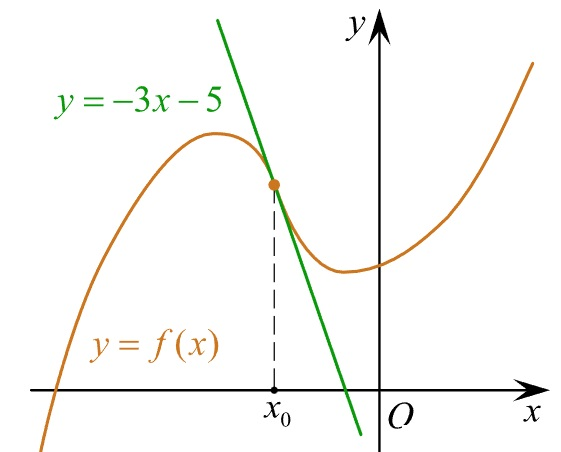
\includegraphics[align=t, width=\linewidth]{\picpath/G112M8C3-1}
		\end{minipage}
		%525702
		\item
		\begin{minipage}[t]{\bodywidth}
			На рисунке изображены график функции \(y=f(x)\) и касательная к этому графику, проведённая в точке \(x_0\). Уравнение касательной показано на рисунке. Найдите значение производной функции \(g(x)=-5f(x)-\dfrac{ 2 }{ 11 }x+\ln3\) в точке \(x_0\).
		\end{minipage}
		\hspace{0.02\linewidth}
		\begin{minipage}[t]{\picwidth}
			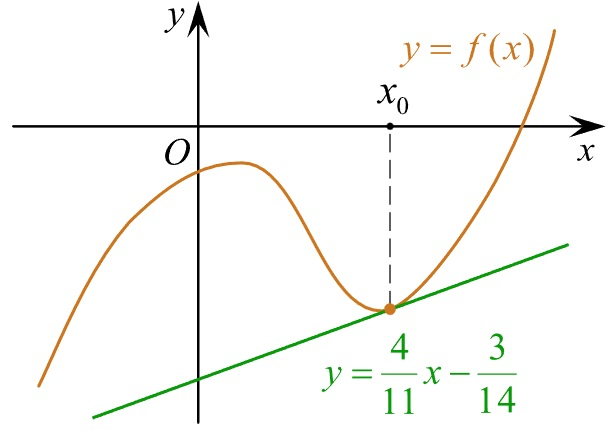
\includegraphics[align=t, width=\linewidth]{\picpath/G112M8C3-2}
		\end{minipage}
		%525691
		\item
		\begin{minipage}[t]{\bodywidth}
			На рисунке изображены график функции \(y=f(x)\) и касательная к этому графику, проведённая в точке \(x_0\). Уравнение касательной показано на рисунке. Найдите значение производной функции \(g(x)=(f'(x)-0,5)\cdot 6\) в точке \(x_0\).
		\end{minipage}
		\hspace{0.02\linewidth}
		\begin{minipage}[t]{\picwidth}
			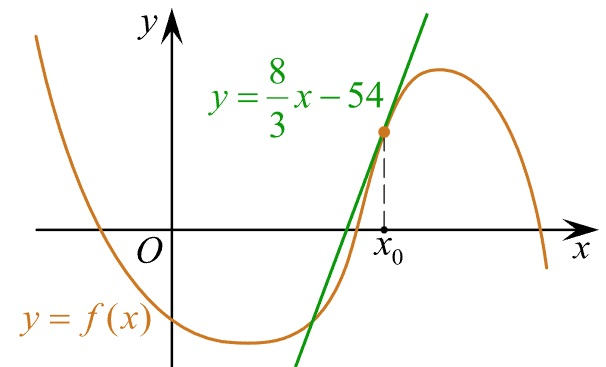
\includegraphics[align=t, width=\linewidth]{\picpath/G112M8C3-3}
		\end{minipage}
		%525703
		\item
		\begin{minipage}[t]{\bodywidth}
			На рисунке изображены график функции \(y=f(x)\) и касательная к этому графику, проведённая в точке \(x_0\). Уравнение касательной показано на рисунке. Найдите значение производной функции \(g(x)=f'(x)-f(x)+3\) в точке \(x_0\).
		\end{minipage}
		\hspace{0.02\linewidth}
		\begin{minipage}[t]{\picwidth}
			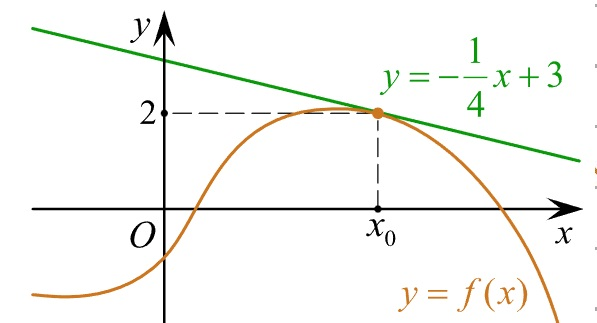
\includegraphics[align=t, width=\linewidth]{\picpath/G112M8C3-4}
		\end{minipage}
		%541816
		\item
		\begin{minipage}[t]{\bodywidth}
			На рисунке изображены график функции \(y=f(x)\) и касательная к нему в точке с абсциссой \(x_0\). Найдите значение производной функции \(f(x)\)в точке \(x_0\).
		\end{minipage}
		\hspace{0.02\linewidth}
		\begin{minipage}[t]{\picwidth}
			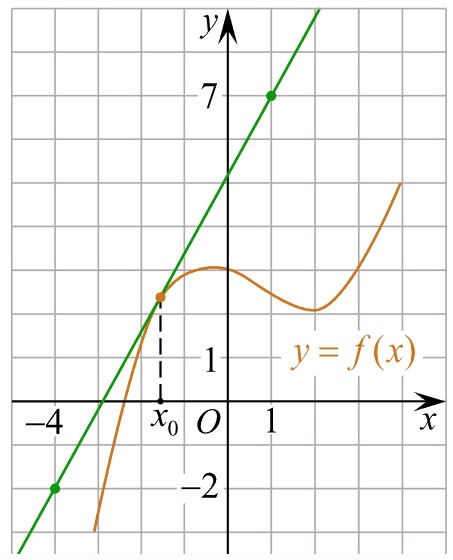
\includegraphics[align=t, width=\linewidth]{\picpath/maksutovM8L4-1}
		\end{minipage}
		%9063
		\item
		\begin{minipage}[t]{\bodywidth}
			На рисунке изображены график функции \(y=f(x)\) и касательная к нему в точке с абсциссой \(x_0\). Найдите значение производной функции \(f(x)\)в точке \(x_0\).
		\end{minipage}
		\hspace{0.02\linewidth}
		\begin{minipage}[t]{\picwidth}
			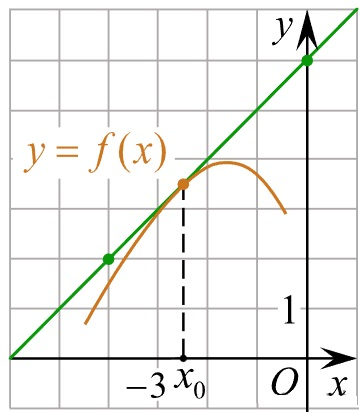
\includegraphics[align=t, width=\linewidth]{\picpath/maksutovM8L4-2}
		\end{minipage}
		%9629
		\item
		\begin{minipage}[t]{\bodywidth}
			На рисунке изображены график функции \(y=f(x)\) и касательная к нему в точке с абсциссой \(x_0\). Найдите значение производной функции \(f(x)\)в точке \(x_0\).
		\end{minipage}
		\hspace{0.02\linewidth}
		\begin{minipage}[t]{\picwidth}
			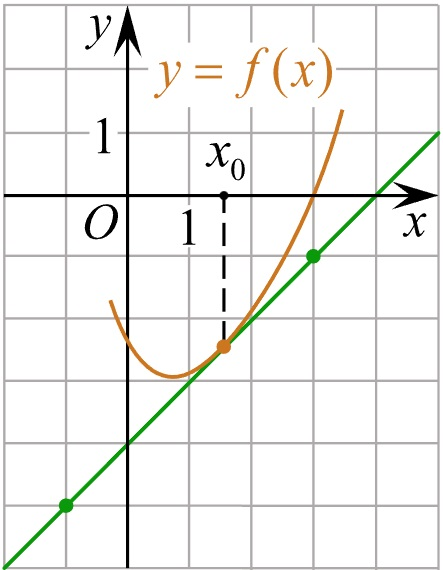
\includegraphics[align=t, width=\linewidth]{\picpath/maksutovM8L4-3}
		\end{minipage}
		
		
		%11-1M8L1 до 6 номера
		\item Вычислить:
		\begin{tasks}(2)
			\task \( \dfrac{-13\sin126\degree}{\sin54\degree} \)
			\task \( \cos^2(-46\degree)+\sin^2(-46\degree) \)
			\task \( \sin^223\degree+9+\cos^223 \)
			\task \( \dfrac{2\sin^221\degree+2\cos^221\degree}{4} \)
		\end{tasks}
		\item Найдите значение выражения: \( \sin\left( \dfrac{\pi}{3}+\alpha \right) \), если \( \cos\alpha=-\dfrac{8}{17} \) и \\ \( \pi<\alpha<\dfrac{3\pi}{2} \).
		%G111M87L2N3
		\item Найдите: %101L1
		\begin{tasks}
			
			\task \( -2\sin\alpha \), если \( \cos\alpha=\dfrac{\sqrt{6}}{5} \) и \( \alpha\in\left( \dfrac{\pi}{2}; \pi \right) \);
			\task \( -\cos\alpha \), если \( \sin\alpha=-\dfrac{5\sqrt{2}}{8} \) и \( \alpha\in\left( \dfrac{3\pi}{2}; 2\pi \right) \);
			\task \( -5\cos\alpha \), если \( \sin\alpha=0,6 \);
			\task \( \sin\left( \dfrac{3\pi}{2}+\alpha \right) \), если \( \sin\alpha=0,6 \) и \( \alpha\in\left( \dfrac{\pi}{2}; \pi \right) \).
		\end{tasks}
		
		\item Найдите наибольшее значение функции \( y=12 \cos x + 6 \sqrt{3} x -2 \sqrt{3} \pi + 6 \) на отрезке \(\left[ 0;\dfrac{ \pi }{ 2 } \right] \).
		\item Найдите наименьшее значение функции \( y=3+\dfrac{5\pi  }{4  }-5x-5\sqrt{2} \cos x \) на отрезке \(\left[ 0; \dfrac{ \pi }{ 2 } \right] \).
		\item Найдите наибольшее значение функции \( y=5 \cos x -6x+4 \) на отрезке \(\left[ -\dfrac{3\pi  }{ 2 };0 \right] \).
		
	\end{listofex}
\end{class}
%END_FOLD

%BEGIN_FOLD % ====>>_ Домашняя работа 2 _<<====
\begin{homework}[number=2]
	\begin{listofex}
		%G111M8L5
		%analog 26784 1-2 V 62785 1-2
		\item Найдите:
		\begin{tasks}
			\task \( -2 \sin \left( \dfrac{ \pi }{ 2 }+\alpha \right) \), если \( \sin \alpha = -0,96 \) и \( \alpha \in (\pi;1,5\pi) \);
			\task \( -4 \cos \left( \dfrac{ 5\pi }{ 2 }+ \alpha \right) \), если \( \cos \alpha = \dfrac{ 7 }{ 25 } \) и \( \alpha \in (1,5\pi; 2\pi) \);
			\task \( 2\sin \left( \dfrac{ \pi }{ 2 }- \alpha \right) \), если \( \sin \alpha = -0,8 \) и \( \alpha \in (1,5\pi;2\pi) \);
			\task \( 5 \cos \left( \dfrac{ 7\pi }{ 2 } + \alpha \right) \), если \( \cos \alpha = \dfrac{ \sqrt{2} }{ 2 } \) и \( \alpha \in (0;0,5\pi) \).
		\end{tasks}
		%11 trigon 4-7
		\item Найдите наибольшее значение функции \( y=15x-3\sin x+5 \) на отрезке \(\left[ -\dfrac{ \pi }{ 2 };0 \right] \).
		\item Найдите наименьшее значение функции \( y=9\cos x +14x +7 \) на отрезке \(\left[ 0;\dfrac{ 3\pi }{ 2 } \right] \).
		\item Найдите наименьшее значение функции \( y=7 \sin x -8x +9 \) на отрезке \(\left[ -\dfrac{ 3\pi }{ 2 };0 \right] \).
		\item Найдите наименьшее значение функции \( y=6 \cos x + \dfrac{ 24 }{ \pi }x+5 \) на отрезке \(\left[ -\dfrac{ 2\pi }{ 3 };0 \right] \).
		%11.5 5-7
		\item Найдите наибольшее значение функции \( y=9x-\ln(9x)+3 \) на отрезке \(\left[ \dfrac{ 1 }{ 18 };\dfrac{ 5 }{ 18 } \right] \).
		\item Найдите наибольшее значение функции \( y=\ln(11x)-11x+9 \) на отрезке \(\left[ \dfrac{ 1 }{ 22 };\dfrac{5  }{22  } \right] \).
		\item Найдите наибольшее значение функции \( y=2x^2-13x+9 \ln x +8 \) на отрезке \(\left[ \dfrac{ 13 }{ 14 }; \dfrac{  15}{ 14 } \right] \).
		%\item Найдите наибольшее значение функции \(  \) на отрезке \(\left[  \right] \).
		%\item Смешав \(55\)-процентный и \(97\)-процентный растворы кислоты и добавив \(10\) кг чистой воды, получили \(65\)-процентный раствор кислоты. Если бы вместо \(10\) кг воды добавили \(10\) кг \(50\)-процентного раствора той же кислоты, то получили бы \(75\)-процентный раствор кислоты. Сколько килограммов \(55\)-процентного раствора использовали для получения смеси?
		\item Имеется два сплава. Первый содержит \(15\%\) никеля, второй --- \(35\%\) никеля. Из этих двух сплавов получили третий сплав массой \(140\) кг, содержащий \(30\%\) никеля. На сколько килограммов масса первого сплава была меньше массы второго?
		%9629
		\item
		\begin{minipage}[t]{\bodywidth}
			На рисунке изображены график функции \(y=f(x)\) и касательная к нему в точке с абсциссой \(x_0\). Найдите значение производной функции \(f(x)\)в точке \(x_0\).
		\end{minipage}
		\hspace{0.02\linewidth}
		\begin{minipage}[t]{\picwidth}
			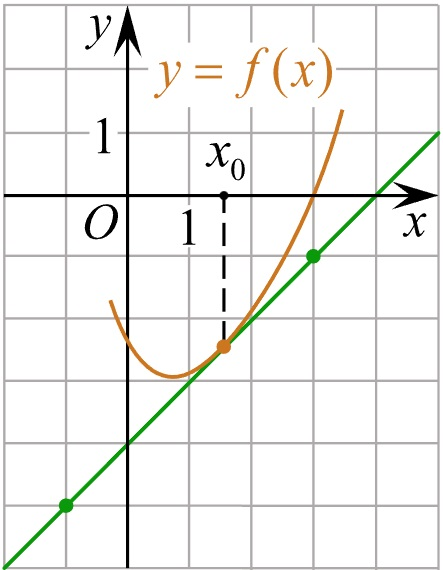
\includegraphics[align=t, width=\linewidth]{\picpath/maksutovM8L4-3}
		\end{minipage}
		%\item 
		%\begin{minipage}[t]{0.45\linewidth}
		%	На рисунке изображены график функции \( y=f(x) \) и касательная к этому графику, проведённая в точке \( x_0=2 \). Найдите значение производной функции \( g(x)=x^2-f(x)+1 \) в точке \( x_0 \).
		%\end{minipage}
		%\begin{minipage}[t]{0.5\linewidth}
		%	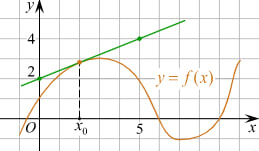
\includegraphics[align=t, width=\textwidth]{\picpath/KuznetsovM8L2_1}
		%\end{minipage}
		%9641
		\item
		\begin{minipage}[t]{0.45\linewidth}
			На рисунке изображены график функции \(y=f(x)\) и касательная к этому графику, проведённая в точке \(x_0\). Уравнение касательной показано на рисунке. Найдите значение производной функции \(g(x)=12f(x)+\dfrac{  6}{13  }\) в точке \(x_0\).
		\end{minipage}
		\hspace{0.02\linewidth}
		\begin{minipage}[t]{0.5\linewidth}
			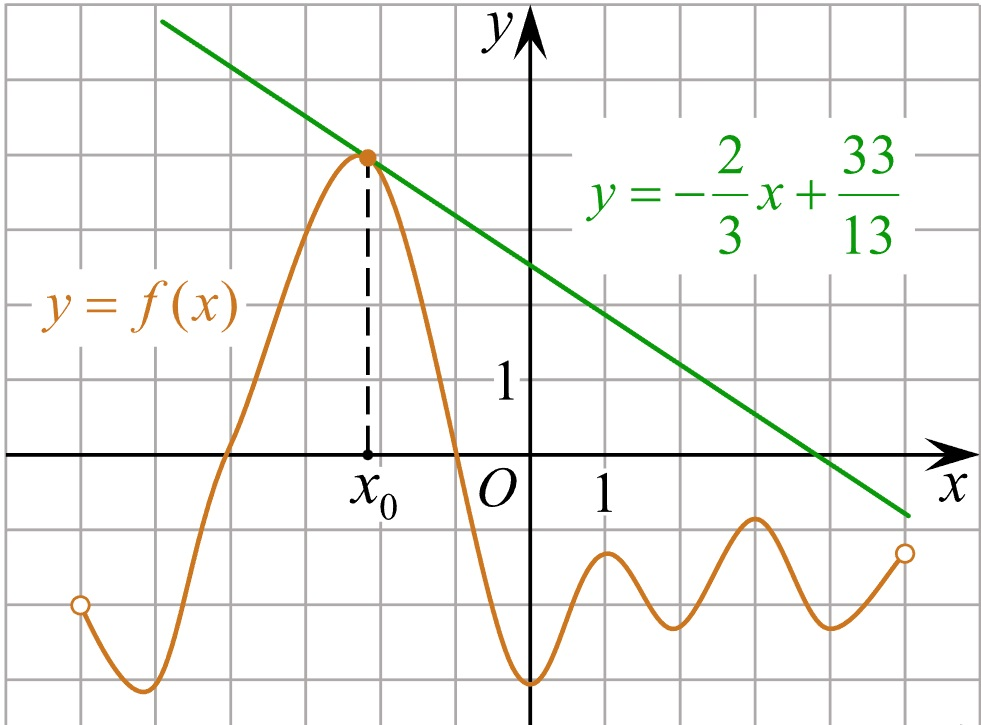
\includegraphics[align=t, width=\linewidth]{\picpath/G111M9H2-1}
		\end{minipage}
		%525446
		%\item
		%\begin{minipage}[t]{0.45\linewidth}
		%	На рисунке изображён график функции \(y=f(x)\) и касательная к нему в точке с абсциссой \(x_0\). Найдите значение производной функции \(f(x)\) в точке \(x_0\).
		%\end{minipage}
		%\hspace{0.02\linewidth}
		%\begin{minipage}[t]{0.5\linewidth}
		%	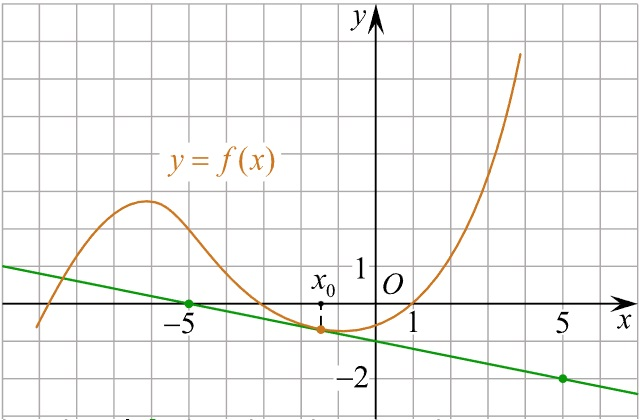
\includegraphics[align=t, width=\linewidth]{\picpath/maksutovM9L2-3}
		%\end{minipage}
		%%525401
		%\item
		%\begin{minipage}[t]{0.45\linewidth}
		%	На рисунке изображён график функции \(y=f(x)\) и касательная к нему в точке с абсциссой \(x_0\). Найдите значение производной функции \(f(x)\) в точке \(x_0\).
		%\end{minipage}
		%\hspace{0.02\linewidth}
		%\begin{minipage}[t]{0.5\linewidth}
		%	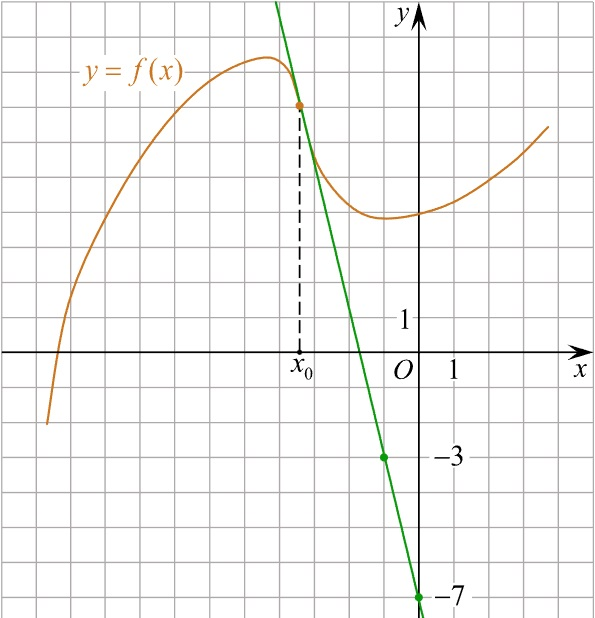
\includegraphics[align=t, width=\linewidth]{\picpath/maksutovM9L2-2}
		%\end{minipage}
		%\item Имеются два сосуда. Первый содержит \(30\) кг, а второй --- \(15\) кг раствора кислоты различной концентрации. Если эти растворы смешать, то получится раствор, содержащий \(34\%\) кислоты. Если же смешать равные массы этих растворов, то получится раствор, содержащий \(46\%\) кислоты. Сколько килограммов кислоты содержится в первом сосуде?
	\end{listofex}
\end{homework}
%END_FOLD

%BEGIN_FOLD % ====>>_____ Занятие 5 _____<<====
\begin{class}[number=5]
	\begin{listofex}
		\item Занятие 5
	\end{listofex}
\end{class}
%END_FOLD

%BEGIN_FOLD % ====>>_____ Занятие 6 _____<<====
\begin{class}[number=6]
	\begin{listofex}
		\item Занятие 6
	\end{listofex}
\end{class}
%END_FOLD

%BEGIN_FOLD % ====>>_ Домашняя работа 3 _<<====
\begin{homework}[number=3]
	\begin{listofex}
		\item Домашняя работа 3
	\end{listofex}
\end{homework}
%END_FOLD

%BEGIN_FOLD % ====>>_____ Занятие 7 _____<<====
\begin{class}[number=7]
	\title{Подготовка к проверочной}
	\begin{listofex}
		\item Занятие 7
	\end{listofex}
\end{class}
%END_FOLD

%BEGIN_FOLD % ====>>_ Проверочная работа _<<====
\begin{exam}
	\begin{listofex}
		\item Проверочная
	\end{listofex}
\end{exam}
%END_FOLD